\documentclass{article}

\input{header}

\title{CSE 5525: Assignment 3}

\author{Jay Himanshu Jivandas}

\date{}


\colmfinalcopy
\begin{document}
\maketitle


\section{Data Statistics and Processing (8pt)}
\paragraph{Instructions:} Use \autoref{tab:data_stats_before} and \autoref{tab:data_stats_after} to describe the data statistics before and after any pre-processing respectively.
Use the T5 tokenizer to report the statistics.
For the statistics after pre-processing, if you did different pre-processing for different models, you need to indicate them separately.
The gray text in each row is there to guide you and should be removed in your submitted report.
Depending on your pre-processing, some numbers may be identical across tables.

\begin{table}[h!]
\centering
\begin{tabular}{lcc}
\toprule
Statistics Name & Train & Dev \\
\midrule
Number of examples & 4225 & 466 \\
Mean sentence length & 10.96 & 10.91 \\
Mean SQL query length & 60.90 & 58.90 \\
Vocabulary size (natural language) & 868 & 444 \\
Vocabulary size (SQL) & 644 & 393 \\
\bottomrule
\end{tabular}
\caption{Data statistics before any pre-processing. Statistics computed using simple whitespace tokenization for word counts and word sets for vocabulary sizes.}
\label{tab:data_stats_before}
\end{table}

\begin{table}[h!]
\centering
\begin{tabular}{lcc}
\toprule
Statistics Name & Train & Dev \\
\midrule
Number of examples & 4225 & 466 \\
Mean sentence length & 23.10 & 23.07 \\
Mean SQL query length & 217.37 & 211.05 \\
Vocabulary size (natural language) & 796 & 470 \\
Vocabulary size (SQL) & 556 & 396 \\
\bottomrule
\end{tabular}
\caption{Data statistics after pre-processing with T5 tokenizer. Natural language inputs are prefixed with ``translate English to SQL:'' before tokenization. The high token-to-word ratio for SQL queries (around 3.6x) is due to T5's subword tokenization splitting SQL identifiers---for example, \texttt{flight\_1.flight\_id} tokenizes to 8 tokens: [\texttt{\_flight}, \texttt{\_}, \texttt{1}, \texttt{.}, \texttt{f}, \texttt{light}, \texttt{\_id}]---and keywords like \texttt{SELECT} split into 3 tokens [\texttt{\_}, \texttt{SEL}, \texttt{ECT}]. Both T5 fine-tuning and from-scratch use identical preprocessing.}
\label{tab:data_stats_after}
\end{table}



\newpage




\section{T5 Fine-tuning and Training From Scratch (8pt)}\label{sec:t5}
\paragraph{Instructions:} Use \autoref{tab:t5_results_ft} and \autoref{tab:t5_results_scratch} to describe your data processing steps (if any) and the implementation details, respectively for the fine-tuned T5 model, and the T5 model trained from scratch.
The gray text in each row is there to guide you and should be removed in the submitted report.
Be clear enough that we can replicate your approach in PyTorch using only your descriptions.

\begin{table}[h!]
\centering
\begin{tabular}{p{3.5cm}p{10cm}}
\toprule
Design choice & Description \\
\midrule
Data processing & Natural language inputs are prefixed with ``translate English to SQL:'' before tokenization. Encoder inputs and decoder outputs are not truncated. The decoder starts with a beginning-of-sequence token, \texttt{<extra\_id\_0>}, and decoder targets include an EOS token at the end during training. No additional preprocessing is done to maintain SQL structure. \\
Tokenization & Inputs to the encoder and decoder are tokenized using the default T5 tokenizer (\texttt{T5TokenizerFast} from \texttt{google-t5/t5-small}). Natural language inputs are prefixed with ``translate English to SQL:'' before tokenization. The decoder has \texttt{<extra\_id\_0>} as the beginning-of-sequence token, and decoder targets are appended with EOS token. Padding is applied at the batch level using \texttt{pad\_sequence} with \texttt{PAD\_IDX=0}. \\
Architecture & Entire pre-trained T5-small model was finetuned without freezing any layers. No architectural modifications are done in fine-tuning. \\
Hyperparameters & Learning rate: 1e-3 (0.001), Batch size: 16, Optimizer: AdamW ($\beta_1{=}0.9$, $\beta_2{=}0.999$, $\epsilon{=}10^{-8}$), weight decay: 0.0, Scheduler: Cosine with 3 warmup epochs, Max epochs: 50, patience epochs: 10, early\_stopping on Record F1, Gradient clipping: max norm 1.0, Generation: Beam search with num\_beams=4, max\_new\_tokens=256, Loss: Cross-entropy on non-padded tokens. \\
\bottomrule
\end{tabular}
\caption{Details of the best-performing T5 model configurations (fine-tuned)}
\label{tab:t5_results_ft}
\end{table}


\begin{table}[h!]
\centering
\begin{tabular}{p{3.5cm}p{10cm}}
\toprule
Design choice & Description \\
\midrule
Data processing & Same as fine-tuning (\autoref{tab:t5_results_ft}). \\
Tokenization & Same as fine-tuning (\autoref{tab:t5_results_ft}). \\
Hyperparameters & Same as fine-tuning (\autoref{tab:t5_results_ft}) except Learning Rate: 1e-4 (0.0001), and initial weights were randomly initialized using T5Config from \texttt{google-t5/t5-small}. Warmup epochs: 15, Max epochs: 100, patience epochs: 40. Early stopping is based on \emph{dev loss} rather than Record F1, since F1 stays flat for many epochs while the model is still learning valid SQL syntax (loss continues to decrease). Gradient clipping with max norm 1.0 was applied to stabilize training with random initialization. \\
\bottomrule
\end{tabular}
\caption{Details of the best-performing T5 model configurations (from scratch)}
\label{tab:t5_results_scratch}
\end{table}


\newpage



\section{Large Language Model (LLM) Prompting (14pt)}\label{sec:llm}

\subsection{In-Context Learning (ICL)}\label{sec:llm:icl}

\paragraph{Instructions:} Provide in \autoref{tab:icl_prompts} the instruction prompt(s) that you used for ICL.

If the prompt you used for zero- and few-shot prompting is identical, except for the examples, there's no need to repeat it.
If you made small modifications between zero- and few-shot, please provide them separately.
For all entries, you need to specify the corresponding values of $k$.




\begin{table}[h!]
\centering
\begin{tabular}{p{1cm}p{12cm}}
\toprule
\textbf{Shot} & \textbf{Prompt} \\
\midrule
    $k{=}0,1,3$ & You are a SQL expert. Translate the following natural language question into a SQL query for a flight database. \\
    & \\
    & \textcolor{ForestGreen}{[Database schema in JSON format describing all tables, columns, and types]} \\
    & \\
    & \textcolor{Blue}{Important: Return ONLY the SQL query with no explanation.} \\
    & \\
    & (Included when $k > 0$:) \\
    & Here are some examples: \\
    & \\
    & Question: [1st example question] \\
    & SQL: [1st example SQL] \\
    & \\
    & Question: [2nd example question] \\
    & SQL: [2nd example SQL] \\
    & \\
    & {[}...till $k$th example{]} \\
    & \\
    & Question: [input question] \\
    & SQL: \\
\bottomrule
\end{tabular}
\caption{Instruction prompts used for zero- and/or few-shot prompting. The same template is used for all values of $k$; the only difference is the inclusion of $k$ examples when $k > 0$. Parts highlighted in \textcolor{ForestGreen}{green} (schema) and \textcolor{Blue}{blue} (task instruction) are ablated in the ablation study (\autoref{tab:ablation_explanation}).}
\label{tab:icl_prompts}
\end{table}


\paragraph{Example selections:} For $k > 0$, we experimented with two example selection strategies: (1) \textbf{random selection}, where $k$ training examples are sampled uniformly at random, and (2) \textbf{similarity-based selection}, where we select the $k$ training examples most similar to the input question based on word overlap (Jaccard similarity over lowercased word sets: $|A \cap B| / |A \cup B|$). Similarity-based selection significantly outperformed random selection (Record F1 0.311 vs.\ 0.113 for $k{=}3$ with Gemma), as it provides the model with structurally relevant examples that share vocabulary and query patterns with the target question.



\newpage



\subsection{Best Prompt and Ablation Study}



\paragraph{Instructions:} Report the best prompt you used in \autoref{tab:best_prompt}.
If the best prompt you used is the same as the one specified in \autoref{tab:icl_prompts}, you can just copy the best prompt and label it.
If it is different (e.g. you designed another prompt that is better), you should clearly describe how you created it and what are the methods you used in the caption.

You will also need to clearly and succintly describe in \autoref{tab:ablation_explanation} the ablation experiments that you performed by removing different parts of the prompt.
For that, you need to first highlight the parts of the prompt that you ablated for each experiment in a distinct color\footnote{\url{https://www.overleaf.com/learn/latex/Using_colors_in_LaTeX}}, as shows the placeholder example in \autoref{tab:icl_prompts}, and second, provide the description by referring to the highlighted part.
When reporting your results in \autoref{tab:results}, you will need to refer to your ablations variants.



\begin{table}[h!]
\centering
\begin{tabular}{p{13.5cm}}
\toprule
\textbf{Prompt (best: $k{=}3$, similarity-based selection)} \\
\midrule
    You are a SQL expert. Translate the following natural language question into a SQL query for a flight database. \\
    \\
    \textcolor{ForestGreen}{[Database schema in JSON format describing all tables, columns, and types in the flight database]} \\
    \\
    \textcolor{Blue}{Important: Return ONLY the SQL query with no explanation.} \\
    \\
    Here are some examples: \\
    \\
    Question: [similar example 1] \\
    SQL: [gold SQL 1] \\
    \\
    Question: [similar example 2] \\
    SQL: [gold SQL 2] \\
    \\
    Question: [similar example 3] \\
    SQL: [gold SQL 3] \\
    \\
    Question: [input question] \\
    SQL: \\
\bottomrule
\end{tabular}
\caption{The best prompt corresponds to the prompt from \autoref{tab:icl_prompts} with $k = 3$ (three-shot) using similarity-based example selection. This configuration provides the database schema (\textcolor{ForestGreen}{green}), explicit output formatting guidance (\textcolor{Blue}{blue}), and the 3 most similar training examples to demonstrate query patterns.}
\label{tab:best_prompt}
\end{table}



\begin{table}[h!]
\centering
\begin{tabular}{p{2cm}p{10cm}}
\toprule
\textbf{Color} & \textbf{Description} \\
\midrule
\textcolor{ForestGreen}{ForestGreen} & Removing the database schema context (ptype=1). The full JSON schema describing all tables, columns, and types is removed from the prompt. Without the schema, the model must rely solely on its pre-training knowledge and the few-shot examples to infer valid table and column names. This tests whether explicit schema information helps the model generate valid column and table references. \\
\midrule
\textcolor{Blue}{Blue} & Removing the task instruction ``Important: Return ONLY the SQL query with no explanation.'' (ptype=2). This instruction constrains the model to output only SQL without natural language explanation. Removing it tests whether the model can still produce clean, parseable SQL output from the role instruction and examples alone. \\
\bottomrule
\end{tabular}
\caption{Ablation variants. Each ablation removes one highlighted component from the best prompt in \autoref{tab:best_prompt} while keeping all other parts unchanged.}
\label{tab:ablation_explanation}
\end{table}



\newpage



\section{Results and Analysis (20pt)}

\paragraph{Quantitative Results:} Use \autoref{tab:results} to report your test and development set results.
Your test results should match with the results on gradescope.
For the development set, you should also report results from experiments you conducted to arrive at your final configuration.
When reporting experiments, you should replace ``variant'' with brief and meaningful descriptions of whatever hyperparameter or setting that you varied.
For ICL, you should specify what is the parameter $k$ used, and what the full model corresponds to. For T5, the full model refers to the best model you described in Section \ref{sec:t5}.
For T5, if you experimented with different design choices, you can add rows specifying the variants and what you tried.
The text in gray is only for example purpose, and should be removed and replaced with your own choices.
You may add more rows if needed.

\begin{table}[h!]
\centering
\begin{tabular}{lcc}
  \toprule
  System & Query EM & F1 score\\
  \midrule
  \multicolumn{3}{l}{\textbf{Dev Results}} \\
  \midrule
  \multicolumn{3}{l}{\textbf{Gemma-2B LLM Prompting}} \\
  Full model ($k{=}3$, similar selection) & 0.00 & 31.08 \\
  Zero-shot ($k{=}0$) & 0.00 & 12.02 \\
  1-shot, random ($k{=}1$) & 0.00 & 6.97 \\
  3-shot, random ($k{=}3$) & 0.00 & 11.30 \\
  \textit{Ablation Studies (from best: $k{=}3$, similar)} & & \\
  \textcolor{ForestGreen}{No schema (ptype=1)} & 0.00 & 14.54 \\
  \textcolor{Blue}{No task instruction (ptype=2)} & 0.00 & 11.49 \\[5pt]
  \multicolumn{3}{l}{\textbf{T5 Fine-tuned}} \\
  Full model (lr=1e-3) & 3.00 & 69.49 \\
  Variant (lr=1e-4) & 2.15 & 60.60 \\[5pt]
  \multicolumn{3}{l}{\textbf{T5 From Scratch}} \\
  Full model (lr=1e-4) & 2.58 & 52.41 \\
  Variant (lr=1e-3) & 0.00 & 11.80 \\
  \midrule
  \multicolumn{3}{l}{\textbf{Test Results}} \\
  \midrule
  ICL & 0.00 & 21.63 \\
  T5 fine-tuning & 0.00 & 63.84 \\
  T5 from scratch & 0.00 & 45.35 \\
  \bottomrule
\end{tabular}
\caption{Development and test results for all models. All scores are percentages. LLM prompting shows performance across shot counts ($k$) and example selection strategies. T5 models show variants with different learning rates. Best configurations are labeled as ``Full model.''}
\label{tab:results}
\end{table}


\paragraph{ICL sensitivity to $k$:} For ICL, please provide a plot of the Record F1 on the development set that the model achieved with different values of $k$. The x-axis should be $k$, and the y-axis the Record F1. The prompts and examples used for this plot should correspond to the ones you described in Subsection \ref{sec:llm:icl}.

\begin{figure}[h!]
\centering
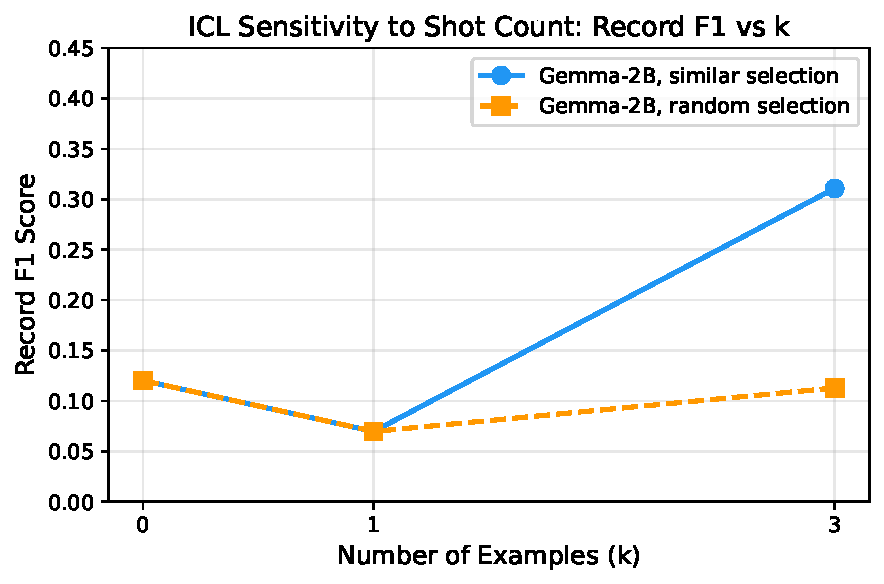
\includegraphics[width=0.8\textwidth]{icl_sensitivity.pdf}
\caption{ICL sensitivity to shot count $k$. With similarity-based selection, performance increases dramatically from $k{=}1$ to $k{=}3$, while random selection shows minimal improvement. Both strategies show a dip at $k{=}1$, suggesting that a single example can mislead the model if it is not sufficiently representative.}
\label{fig:icl_sensitivity}
\end{figure}

\newpage

\paragraph{Qualitative Error Analysis:} Conduct a detailed error analysis for each of the three models. Identify common error types and discuss possible reasons for these errors in \autoref{tab:qualitative}.

You must identify at least three classes of errors for the queries, and use examples to illustrate them.
It must be clear what model makes the errors you are analyzing.
If you identified the same type of error for different models, you don't need to duplicate the descriptions, but you need to clearly specify an example for each of the model, indicate the statistics for each model, and specify to which model each statistics correspond to.
You may add more rows to the table.


\begin{landscape}
\begin{table}
  \centering
  \small
  \begin{tabular}{p{2.2cm}p{2cm}p{5.5cm}p{5.5cm}p{5.5cm}}
    \toprule
    \textbf{Error Type} & \textbf{Relevant Models} & \textbf{Example Of Error} & \textbf{Error Description} & \textbf{Statistics} \\
    \midrule
    Invalid column references & All models &
    ICL: \texttt{no such column: airport\_1.city\_name} \newline
    T5-ft: \texttt{no such column: fare.round\_trip\_cost} \newline
    T5-scr: \texttt{no such column: flight\_1.departure\_city} &
    The model generates SQL referencing columns that do not exist in the database schema. The ICL model frequently hallucinates plausible but non-existent column names. T5 models also produce invalid references, especially for less common query patterns involving fares, restrictions, and flight stops. &
    ICL (3-shot similar): 98/466 \newline
    T5-ft: 67/466 \newline
    T5-scr: 137/466 \\
    \midrule
    Incorrect or missing table joins & All models &
    Gold: \texttt{flight\_1.from\_airport = airport\_service\_1.airport\_code AND airport\_service\_1.city\_code = city\_1.city\_code} \newline
    ICL pred: \texttt{flight\_1.from\_airport = city\_1.city\_name} &
    Models fail to correctly join tables through intermediate linking tables. The flight database requires multi-hop joins (e.g., flight $\rightarrow$ airport\_service $\rightarrow$ city), but models often try to directly join non-adjacent tables or omit necessary intermediate joins entirely. &
    ICL: ${\sim}$150/466 \newline
    T5-ft: ${\sim}$45/466 \newline
    T5-scr: ${\sim}$90/466 \\
    \midrule
    SQL syntax errors & ICL, T5-scr &
    ICL: \texttt{near ")": syntax error} \newline
    ICL: \texttt{incomplete input} \newline
    T5-scr: \texttt{near "1": syntax error} &
    The model generates syntactically invalid SQL with unmatched parentheses, missing clauses, or truncated queries. This is especially common in ICL where the model may produce extraneous text or fail to complete the query before hitting the max token limit. T5-ft rarely produces syntax errors due to learning SQL structure during fine-tuning. &
    ICL: 15/466 \newline
    T5-scr: 8/466 \newline
    T5-ft: 0/466 \\
    \midrule
    Non-existent tables & ICL &
    ICL: \texttt{no such table: ground\_transportation} \newline
    ICL: \texttt{no such table: car} &
    The ICL model hallucinates table names that do not exist in the schema, drawing on general SQL knowledge rather than the provided schema. For example, it generates \texttt{ground\_transportation} instead of the correct \texttt{ground\_service} table. T5 models rarely exhibit this error since they learn the correct table names from training data. &
    ICL: 12/466 \newline
    T5-ft: 0/466 \newline
    T5-scr: 2/466 \\
    \bottomrule
  \end{tabular}
  \caption{Qualitative error analysis on the dev set for all three models. Error counts for ``Invalid column references'' and ``SQL syntax errors'' are computed by pattern-matching on error messages. Counts for ``Incorrect or missing table joins'' are estimated by manual inspection of a sample of queries that produced wrong results but no SQL errors.}
  \label{tab:qualitative}
\end{table}
\end{landscape}



\end{document}
